\documentclass[border=4pt]{standalone}

% --- packages (mirror these in transformer.meta.json "requires") ---
\usepackage{tikz}

% --- palette (canonical source: reference/color-palettes/color-palettes.md; light variant) ---
\definecolor{otblue}{HTML}{0072B2}
\definecolor{otorange}{HTML}{E69F00}
\definecolor{otteal}{HTML}{009E73}
\definecolor{otpurple}{HTML}{CC79A7}
\definecolor{otgray}{HTML}{5A5A5A}

\begin{document}
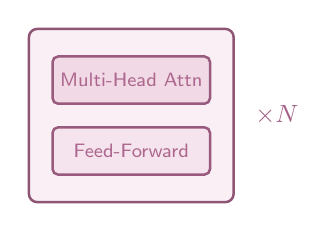
\begin{tikzpicture}[line width=0.9pt]
  % transformer block
  \filldraw[draw=otpurple!70!black, fill=otpurple!12, rounded corners=3pt] (0,0) rectangle (2.6,2.2);
  % multi-head attention sub-layer
  \filldraw[draw=otpurple!75!black, fill=otpurple!28, rounded corners=2pt] (0.3,1.25) rectangle (2.3,1.85);
  \node[font=\sffamily\scriptsize, text=otpurple!85!black] at (1.3,1.55) {Multi-Head Attn};
  % feed-forward sub-layer
  \filldraw[draw=otpurple!75!black, fill=otpurple!20, rounded corners=2pt] (0.3,0.35) rectangle (2.3,0.95);
  \node[font=\sffamily\scriptsize, text=otpurple!85!black] at (1.3,0.65) {Feed-Forward};
  % stacked-layer repeat indicator
  \node[font=\sffamily\small\bfseries, text=otpurple!80!black] at (3.15,1.1) {$\times N$};
\end{tikzpicture}
\end{document}
